\section{N2Sky Architecture}\label{TheN2SkyArchitecture}

\subsection{Current Architecture Analysis}\label{CurrentArchitectureAnalysis}

Current N2Sky architecture a monalitic stand alone application. It was heavily maintainable and not scalable. Before proposing the new architecture design it is important to find the weak parts of the current application and define what functionality is still possible to reuse in order gain new functionality with a reasonable time.  

\subsubsection{Architecture design}\label{Architecturedesign}

The current N2Sky design based on RAVO architecture \cite{ravo}, which extends default SPI stack. SPI stack contains Infrastructure as a Service (IaaS), Platform as a Service (PaaS) and Software as a Service (SaaS). The architecture had a two phases of integration.  In the first phase the SPI was extended and applied to N2Sky application. On the last phase all mandatory components were implemented and integrated as it presented in figure \ref{fig:current_arch}.

\begin{figure}[htbp]
\begin{center}
  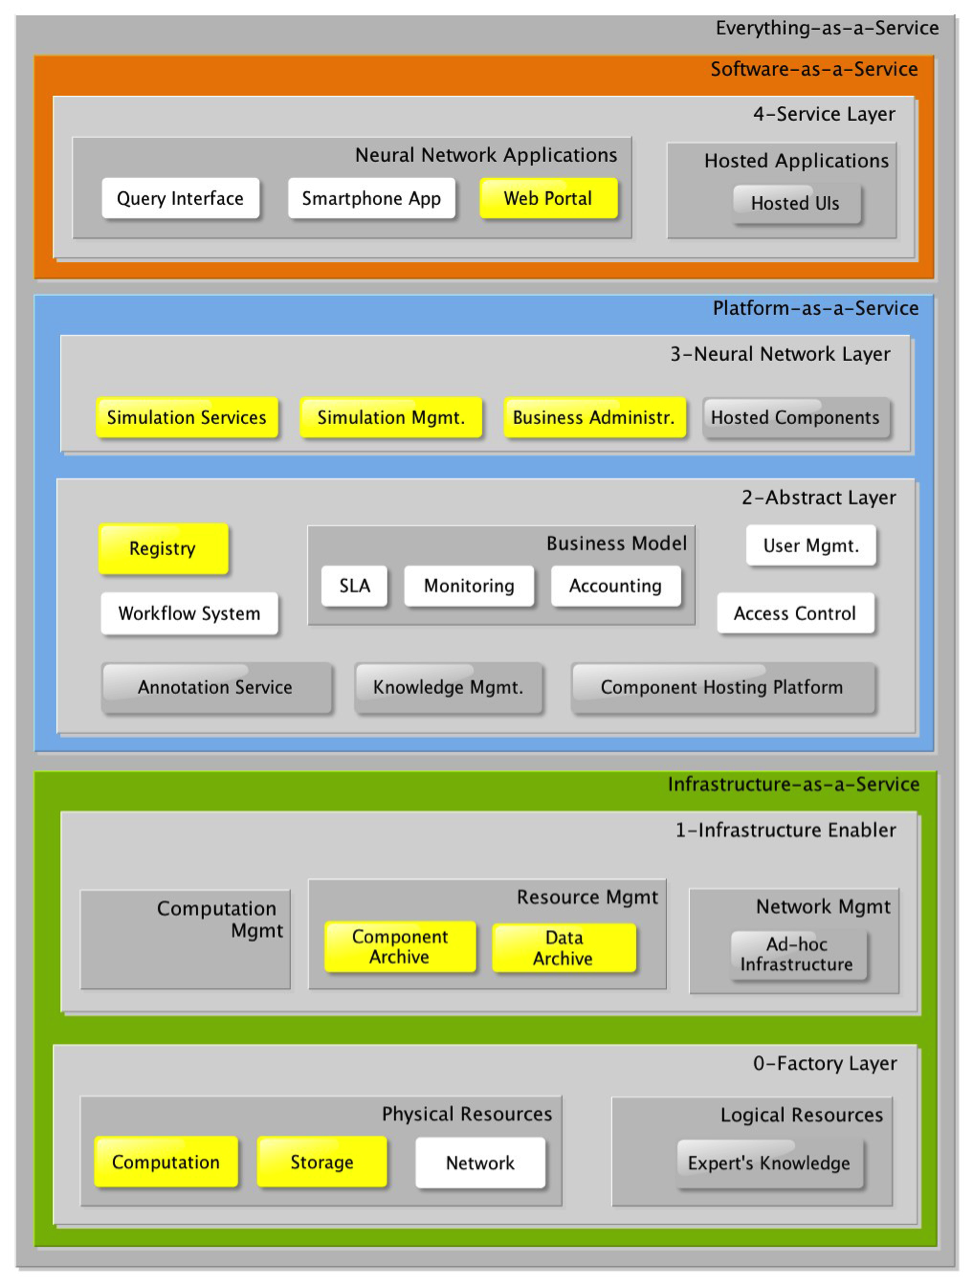
\includegraphics[width=\linewidth]{components/2/current_arch.png}
  \caption{Current N2Sky architecure}
  \label{fig:current_arch}
\end{center}
\end{figure}

Every service represents the particular layer:
\begin{itemize}
\item \emph{IaaS layer}  responsible for managing  the resources. It contains the logical and physical resources of N2Sky components as well as infrastructure enabler like protocols, procures etc. 
\item \emph{PaaS layer}, which provides an access to resources via API. In previous N2Sky system it served as a domain-independent tool. It also contains the neural network layer.
\item \emph{SaaS} is a service, which container the User interfaces (UIs).
\end{itemize}

Everything as a service is a good idea, but build upon it the layered architecture could cause some issues. Since every layer depending on the layer above there are possibility if the services from bottom layer goes then the application is not usable at all. 

Besides stand-alone-application design, which was implemented, another one issue is encapsulation. Since every service need to communicate with other services via API the order of layers could be violated. This problem can cause not only security issues, bus also consistency, namely it can breaks the desired workflow process.

Unfortunately it is impossible to distribute the services, since they are all coupled together into collections of layers.  

\subsubsection{Components}\label{Components}

N2Sky was an imposing application, which contained multiple services and was working as whole. Following main components were listed in N2Sky:

\begin{itemize}
\item \emph{The component archive} was responsible for storage and file management.
\item \emph{The data archive} is the component, which managed the neural network specific resources in XML and JSON formats. 
\item \emph{The registry}, which was a base component of N2Sky architecture. This component was responsible for searching of services within the cloud.  It also contained instructions and rules, which were used by users. 
\item \emph{Monitoring} was divided into two subcategories: business activity monitoring (BAM), which was gather the business data and technical monitoring, which was responsible for environment monitoring and performance statistics. 
\end{itemize}

Considering that the registry is a central components, because it responsible for services management, it can slow down the whole process. All requests are going throw this services. If the services is not accessible or high latency or waiting time occurs, the UI as well as API services would be not available.

It would be great to have the same service, but distribute them on multiple servers. Every service in previous version of N2Sky is  gigantic, it is possible to divide services into microservices and incapsulate sensible components from public access.

\subsubsection{Implementation}\label{Implementation}

The previous version of N2Sky is fully written on Java using Spring framework and java servlets. The Tomcat server was used, because of the Java programming language. The  Java Spring framework is good for enterprise application, but the N2Sky needs lots of computations so the  high-end super computers is necessary pre-requirement in this case. 

Unfortunately it is impossible to map the current architecture into micro-services approach. Only one solution is to make replicas of the application, but then the sessions and data consistency hast to be tracked in every replica. 

The mobile application of the N2Sky is build with raw HTML5 and JavaScript. Today, looking on this mobile application it is close to impossible to maintain it. Nevertheless,  the mobile version is also wrapped into layered architecture and in implementation it is still one project. The solution to this problem is responsive design. The responsive design could be fully adaptive to multiple devices from desktop PCs to mobile with a small screen resolution.

The whole system is deployed on Amazon Web Services (AWS), which is good if the owner has enough resource to keep it working. Best solution would be to have a dedicated server with a real physical memory and computational abilities. 


\subsubsection{Usability and user experience}\label{Usabilityanduserexperience}



\subsection{Redesign motivation}\label{Redesignmotivation}

Application redesign is a project, which takes a lot of work. But at some point every designer faced a refactoring project. It has a lot to do with user experience. Bad user experience will make users stop use an application and leave negative feedback on application in general. 

\subsubsection{Redesign Process }\label{Redesign Process}

There is data, information and user experience of previous version of N2Sky to work with. Making redesign it is already known who the users are and what they are trying to achieve.  Using this information it is possible to build an aims for a future user interface and user experience.


\begin{description}

\item[Finding problems.]  There are multiple problems with the application. One of the most crucial is that user interface is not intuitive understandable. 
\begin{figure}[htbp]
\begin{center}
  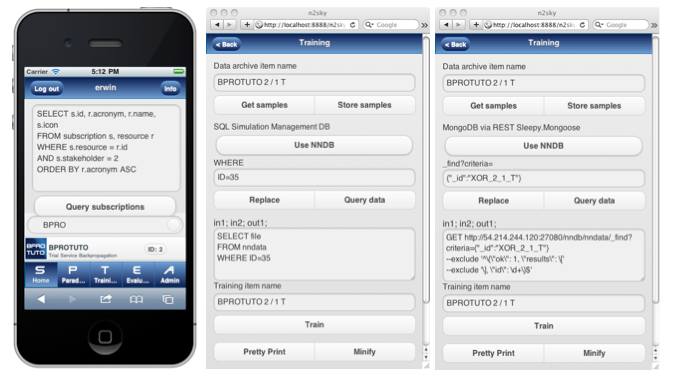
\includegraphics[width=\linewidth]{components/2/old_arch.png}
  \caption{Current N2Sky User Interface}
  \label{fig:old_arch}
\end{center}
\end{figure}


After signing in user getting subscription form, paradigm service and paradigm metadata views without any field description. Small titles unfortunately not always self-describing. Application in general oriented on the group of users, who are came from IT area. In some forms they can type queries, but the fields are not type safe and there is no autocomplete.
Representation of neural networks trained model is not readable. The model represented as a raw JSON or XML file, user can not download it. The last point is a design in general that does not look up-to-date and user attractive. 


\item[User interviews and Questionnaire.]
User insights are very important. It helps to understand a nature of the problem. But if user find something confusing, the interviewer need to dig deeper to stress the importance of particular insight. Unfortunately there were no analytics data and any reviews regarding UI and UX, so with a small group of colleges the current UI of N2Sky was reviewed. 
The following questions were derived (Q1-Q5): 


\begin{itemize}
\item Q1: "How N2Sky can help you with a developing of your neural network?"
\item Q2: "What was the most difficult part by creating a new model?"
\item Q3: "Did you face any problems during spawning your neural network? If yes, then what kind?"
\item Q4: "Did you find out something new, when other users were performing testing against your neural network?"
\item Q5: "What did you miss during using an N2Sky?"
\end{itemize}	

There were 5 students interviewed. All students were together in one group. Summarise answers (A1-A5) according to questions (Q1-Q5): 

\begin{itemize}
\item A1: N2Sky gives possibility to test the own neural network. Unfortunately, if the user does not have a neural network it is impossible to test the application.   
\item A2:  User face difficulties during creation of the new neural network model. User interface user technical jargon and it is not intuitively understandable.  
\item A3:  Spawning a neural network was pretty clear process, but it was not really clear if neural network ready to use or not.
\item A4:  Logging of the training data is very useful. The neural network owner can see how his network behaves with a different training and testing data.
\item A5:  User wants perform testing and training on already existing neural networks. 
\end{itemize}	


\item[Current application design mapping.]

After studying the answers it is possible to highlight weak parts of application. This approach will show a big picture of the current application design:

\begin{itemize}
\item Arbitrary user needs to know multiple technologies and programming languages just simply to reuse existing neural network. 
\item Too much information on every view. The purpose of view is overloaded. Each view has too much functionality, which makes user to loose a focus.
\item Application works relatively slow. Even if there some processes behind happening, the user des not know it.
\end{itemize}

Important is to face the problems, but does not "reinvent the wheel".  As \hl{Joel Spolsky the} founder of Netscape and CEO of Stack Overflow said, ??throwing away the whole program is a dangerous folly?. That is why it was decided to consider the problems of current N2Sky design and reuse working ideas in refactored system

\item[Application Maintenance.]
N2Sky was monolithic standalone application, which included all services in one and was deployed as a whole. The application was not distributed.  In case if one of the services doesn?t work correct, the whole application is not usable. 
Originally the previous version of N2Sky was written fully on Java. There were hundreds classes, providers and services in one project. Developer will spend hours to maintain this kind of project. To find an issue in a big application is always a challenge.  Small changes are causes a subsequence changes. If the software breaks after change, than it will additional high effort to fixed it. As Robert Cecil Martin wrote in his book ?Clean Code?: ?The code is hard to understand. Therefore, any change takes additional time to first reengineer the code and is more likely to result in defects due to not understanding the side effects? \hl{[https://www.amazon.com/Clean-Code-Handbook-Software-Craftsmanship/dp/0132350882]}.  He categorizes this kind of code into ?Smell? code. Unfortunately N2Sky from maintain perspective had all problems, which Mr. Martin

That is why N2Sky is shifted from monolithic system to container based system with an independent micro services which located on cloud environment. 
The frontend and frontend services are lightweight and easy to maintain parts of the big application. If something goes wrong, the developer knows exactly where is the problem. It is close to impossible to break something else during fixing because of independence of services. 
Additionally there are monitoring and alerting systems which are supporting developers during maintenance.  Early it was not possible to say if application works correctly or even it still running. Users could get a bad experience while they using an application in case if it does not work correctly. But now it is possible not only notify an application administrator about some problems, but also to predict potential threads. 
\end{description}


\subsubsection{Refactoring the User Interface}\label{Refactoring the User Interface}

User Interface (UI), an abbreviation of user interface, allows the interaction of a user with a program through graphical visualization made by text, icons, buttons and pictures. While deciding the design of a user interface there are some highly recommended features also known as heuristics, which was invented by hl{Jakob Nielsen}. It was decided to apply the following 10 general principals of interaction design to N2Sky:

\begin{description}
\item[Simple and natural dialogue.]  N2Sky will have an simple UI which is understandable for any user, even if the user is not an expert. Every icon and every navigation or action button will be self-describing. The application will follow the slogan ?less is more?. No more overloaded views. The idea of N2Sky UI design is that one particular view is responsible for one particular function or group of functions which a coupled tight together.
\item[Speak the users language.] Developing N2Sky was concentrated on user perspective. There is no technical jargon for arbitrary user.
\item[Minimize user memory load.] There is no multiple options, functions or menus on one view. There is also no multiple ways to do the same thing. N2Sky teach user how to make things done with a one existing and convenient workflow. 
\item[Consistency.] N2Sky has similar layouts, fonts, colors, icons types structures and organization throw entire application. The user should get the same visual experience on every view.
\item[Feedback.] Every action, process or even error will be notified. User will know exactly what is happening with a system with clear and understandable messages.
\item[Clearly marked exits.]  Every push to action button has short and clear caption.
\item[Shortcuts.] N2Sky has multiple user types. One of the types is the expert users, which are advanced user in neural network and artificial intelligence topics. For this kind of user is provided more technical jargon, but this UI is separated with an arbitrary users.  
\item[Good error messages.] Every notification is clear inclusive an error massage if occurs. Every message has a prices and simple description.
\item[Prevent errors.] In N2Sky implemented logical structure of UI components. There are constrains which are helps user in workflow. For example user will always get a default value of any input.
\item[Help and documentation.] N2Sky will have tutorials that describe the user workflow. The expert users will also get a API documentation with a detailed description and sample requests. 

\end{description}

Each and every one of these heuristics is connected to a crucial idea that is usability. By mentioning this idea, a straightforward relation with the UX follows since this is also one of the key concept that grows along the rapid development of technology. UX is known as user experience and it describes the perspective and feelings a user gets when interacting with product. It deepens into such aspect as the users inner circumstances and the nature of the created design. The goal is to achieve such a system that offers distinguished user experience and accomplishes the most of aspects. As above mentioned, usability.  \hl{(1)}
Putting both of UI and UX in a comparison, to all appearances the user interface is the target on the appearance and functionality of the product and its tangible details.  Furthermore, the user experience is the general experience that the user manages throughout the whole use.   \hl{(2)}
UI will concentrate on the appearance and design of the product, rather than the functionality. The intent of it relies in the visual design and layout. UI covers issues such as how a button is supposed to look like, how the errors are going to appear or is it visually comprehensible meaning which colors or font type shall be used for a better perceptibility of the product.  \hl{(6)}
UX points its focus on the involvement of the user while interacting. It is measured by a variety of tests and researches done to achieve a higher satisfaction on the users side.  \hl{(4)}
Though their differences, the only matter which relates both UI and UX is their priority, in other words, the user. When expanding the concept of both these definitions it can be concluded that one co-exists with the other. There would not be user interface without user experience and vice versa. 

 \hl{TODO // CHECK MERSI DOKU}

\subsubsection{Advanced project management}\label{Advanced project management}

In order to make N2Sky competitive on the market, the modern approach in planning of the project has to be done. Today the most common and effective way in development and planning is well-constructed Functional Requirements Specification (FRS), which helps to estimate effort and advice in the future planning. 

FRS is a document that defines functionality, which application or some parts of application must perform \cite{wiki:frs}. N2Sky is sociotechnical system, meaning that is strongly interacts with humans. 

FRS for N2Sky is described in natural language with formal methods in order to establish specifications between development process and end-user consuming. Ever N2Sky module has FRS, which is explicit and points on system functionality. A good FRS must be unambiguous, consistent and correct \cite{frs_1}.  
 
 The formal or semi-formal methods are serving for analysing and validating FRS. The main purpose of  that to limit interpretation errors. The problem occurs when FRS is fully written in natural language, when designers does not have required technical knowledge in order to use other languages. One of  the typical solution is defects detection technics, which require some effort from designer \cite{frs_3}. 
 
In N2Sky some methods and technics were applied in order to make specification clean and clear as possible. Despite that in FRS will be always some parts which are leading to misunderstanding \cite{frs_1}.
  
FRS is a part of engineering phase. Following qualities for N2Sky were defined and applied during this phase \cite{frs_4} as it shown in ``Fig.~\ref{fig:frs_req}'' :
\begin{itemize}
\item Correct
\item Unambiguous
\item Complete
\item Consistent
\item Ranked for importance and/or stability
\item Verifiable
\item Modifiable
\item Traceable 
\end{itemize}


\begin{figure}[htbp]
\begin{center}
  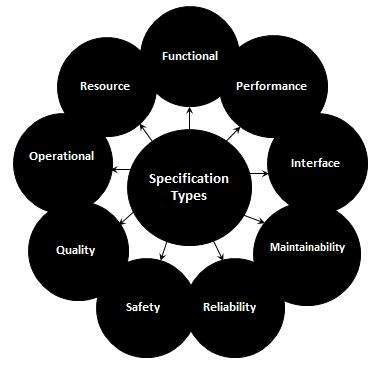
\includegraphics[scale=0.75]{components/4/pics/frs_req.jpg}
  \caption{Applied on N2Sky  Requirement Specification Quialities}
  \label{fig:frs_req}
\end{center}
\end{figure}


\subsubsection{User Roles}\label{User Roles}

In order to make the N2Sky user interface understandable for arbitrary users as well as professional for advances users, it was decided to separate the user roles. Every user role has own way of interaction with the application.

Every user has some specific area within he works. For example, just registered user does not need to know the current environment monitoring information. These restrictions were motivation to create some user roles in order to restrict of grand some functionality of N2Sky as it shown on ``Fig.~\ref{fig:userroles}''.

\begin{figure}[htbp]
\begin{center}
  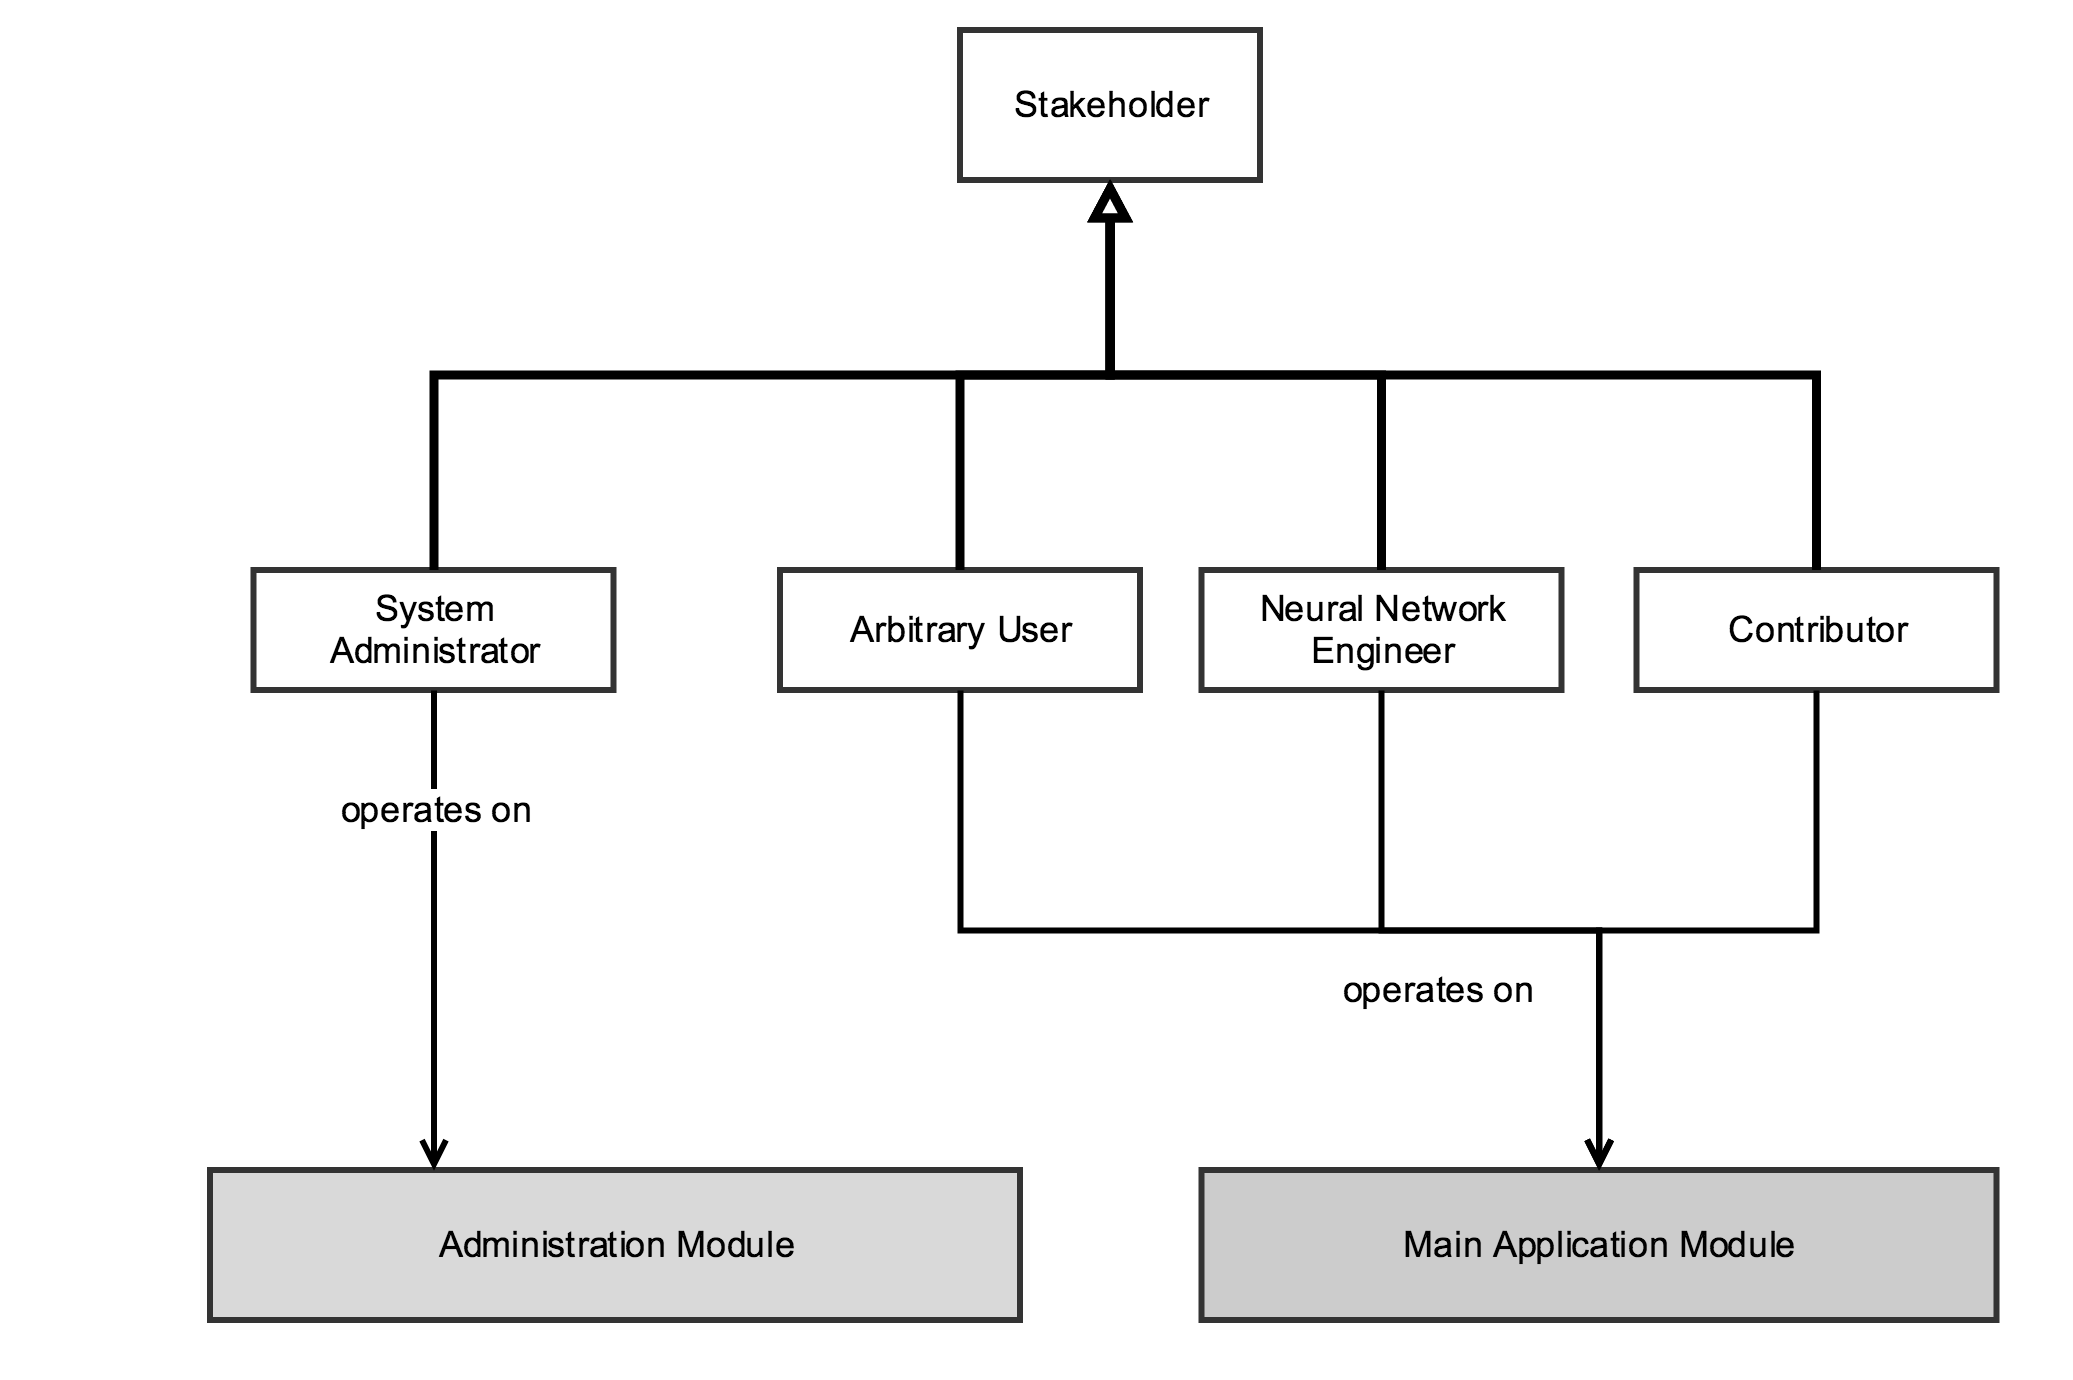
\includegraphics[width=\linewidth]{components/4/pics/users.png}
  \caption{User roles hierarchy and modules where they operating on (marked grey)}
  \label{fig:userroles}
\end{center}
\end{figure}

\begin{itemize}
\item \emph{Arbitrary User.}  The Arbitrary User a user, who does not have a deep knowledge of the neural network field or know any programming language. His main purpose is not a contribution, but the usage already existing neural networks and trained models. The main goal of the arbitrary user is to study neural networks within N2Sky platform. The arbitrary user can also evaluate the trained models or execute training against existing neural networks. This kind of user does not have to use his own training data, he just wants to see the behavior of neural networks. The arbitrary user can be converted to Neural Network Engineer user if he has enough knowledge of it. 
\item \emph{Neural Network Engineer.} The Neural Network Engineer is an arbitrary user. The Neural Network Engineer has an access only to his own dashboard and publicly available resources on the main application module. He can perform the semantic search for available neural network paradigms and use them. This user can create own neural network instance from existing neural network paradigm. He can also train the running neural network instances and evaluate their trained models. This user can share his trained neural network by making it public. 
\item \emph{Contributor.} The Contributor is an expert user, which has enough knowledge and experience to create his own neural network. This user can create neural network paradigms using the ViNNSL template schema and publish them on N2Sky. This user can deploy neural networks on the N2Sky environment as well as on his own environment by providing training and testing endpoints. The goal of the contributor is the study how his networks will behave with different network structures, input parameters and training data that is provided by other users.
\item \emph{System Administrator.} System Administrator is a user who has a full access to the application including environment management, monitoring and alerting features. The administrator can manage OpenStack and Cloudify instances. He also can shadow any N2Sky user to observe the application from other perspectives. The administrator has access to all dashboards in every module.
\end{itemize}


\subsubsection{User Main Functions}\label{User Permissions}

In more detailed overview of user roles it is possible to define permission and main functions.
Permissions describes users allowed page view. If user has access to particular page view the main user function can be defined. 
The main user function characterise allowed behaviour on particular page view. 

As it was mentioned in previous chapter,  N2Sky is an modular application. Permissions and main functions of Administration Module and N2Sky Main Application Controller, which is a part of Main Application Modules, described in Table \ref{table:admin}.

\begin{table}[]
\resizebox{\textwidth}{!}{%
\begin{tabular}{|l|c|c|c|c|c|c|c|c|}
\hline
\multicolumn{1}{|c|}{User Role} & \multicolumn{2}{c|}{\textbf{Administration Module}}          & \multicolumn{2}{c|}{\textbf{N2Sky Main Application Controller}}      \\ \hline
\multicolumn{1}{|c|}{\textbf{}} & \textbf{OpenStack Management} & \textbf{Cloudify Management} & \textbf{Neural Networks Management} & \textbf{Trained Models Management} \\ \hline
System Administrator            & \textbf{+}                    & \textbf{+}                   & \textbf{+}                          & \textbf{+}                            \\ \hline
Moderator                       & \textbf{-}                    & \textbf{-}                   & \textbf{+}                          & \textbf{+}              \\ \hline
Consumer                        & \textbf{-}                    & \textbf{-}                   & \textbf{-}                          & \textbf{-}                            \\ \hline
Developer                       & \textbf{-}                    & \textbf{-}                   & \textbf{-}                          & \textbf{-}                               \\ \hline
Contributor                     & \textbf{-}                    & \textbf{-}                   & \textbf{-}                          & \textbf{-}                    \\ \hline
\end{tabular}%
}
\caption{User Roles main functions considering "Administration Module" and "N2Sky Main Application Controller". 
"+" for allowed, "-" for disallowed}
\label{table:admin}
\end{table}

System Administrator has permissions to all components. Moderator has access only to N2Sky Main Application Controller. Since both of this user roles extending Contributor user role, the permissions for main application module are also granted.

Consumer, Developer and Contributor user roles have no access to any administration parts of N2Sky. This users do not have any main function in this area, but they can operate N2Sky Main Application Module as it shown on Table \ref{table:main}.

\begin{table}[]
\resizebox{\textwidth}{!}{%
\begin{tabular}{|l|c|c|c|c|}
\hline
\multicolumn{1}{|c|}{User Role} & \multicolumn{4}{c|}{\textbf{N2Sky Main Application Module}}                                                                                    \\ \hline
\multicolumn{1}{|c|}{\textbf{}} & \textbf{Paradigm Creation} & \textbf{Neural Networks Creation} & \textbf{Neural Network Training} & \textbf{Training Models Evalutaion} \\ \hline
System Administrator            & \textbf{-}                 & \textbf{-}                        & \textbf{-}                       & \textbf{-}                          \\ \hline
Moderator                       & \textbf{-}                 & \textbf{-}                        & \textbf{-}                       & \textbf{-}                          \\ \hline
Consumer                        & \textbf{-}                 & \textbf{-}                        & \textbf{+}                       & \textbf{+}                          \\ \hline
Developer                       & \textbf{+}                 & \textbf{+}                        & \textbf{+}                       & \textbf{+}                          \\ \hline
Contributor                     & \textbf{-}                 & \textbf{+}                        & \textbf{+}                       & \textbf{+}                          \\ \hline
\end{tabular}%
}
\caption{User Roles main functions considering "N2Sky Main Application Module". 
"+" for allowed, "-" for disallowed}
\label{table:main}
\end{table}

As it was mentioned before System Administrator as well as Moderator has access to N2Sky Main Application Module, but they do not have a main function there. On the other hand all user roles, which are extending consumer can contribute in a N2Sky Main Application Module, except Consumer itself. Consumer has access to all page views on this module, but he has another purpose. 



\subsection{Novel N2Sky Architecture}\label{Contemporary N2Sky Architecture}

N2Sky is a simulation platform, which allows all involved stockholders to use it for computational purposes. In order to achieve high performance and scalability, it was decided to use the microservices architecture. This approach is used not only for backend services but also with frontend and its services.

The user-centered design is a fundamental requirement for N2Sky. Looking back on past experiences with the application, there were identified the real capabilities and needs of users. N2Sky was moved from a complex monolithic system to an easily understandable application. Every interested user without having a deep knowledge in the neural network field can freely use N2Sky.  The goal was to save and gain the current functionality of the application and decrease the visual complexity of it. 

\subsubsection{Cloud infrostructure}\label{Cloud infrostructure}


Upon the N2Sky microservices the the load balancer located, which includes shared cloud resources. Since in N2Sky environment needs to support thousands of Docker containers \cite{docker} simultaneously, only container orchestration like Cloudify \cite{cloudify} with a microservices architecture can perform this.  Cloudify is a container orchestration tool, which provides communication between cloud platforms and manages container deployment and execution. Docker container is a operating-system-level virtualization. Containers technology used across entire system from frontend and services to monitoring and alert management system. 

The novel N2Sky architecture can be scaled horizontally as well as vertically on demand as it presented in figure \ref{fig:newarch}.

\begin{figure}[htbp]
\begin{center}
  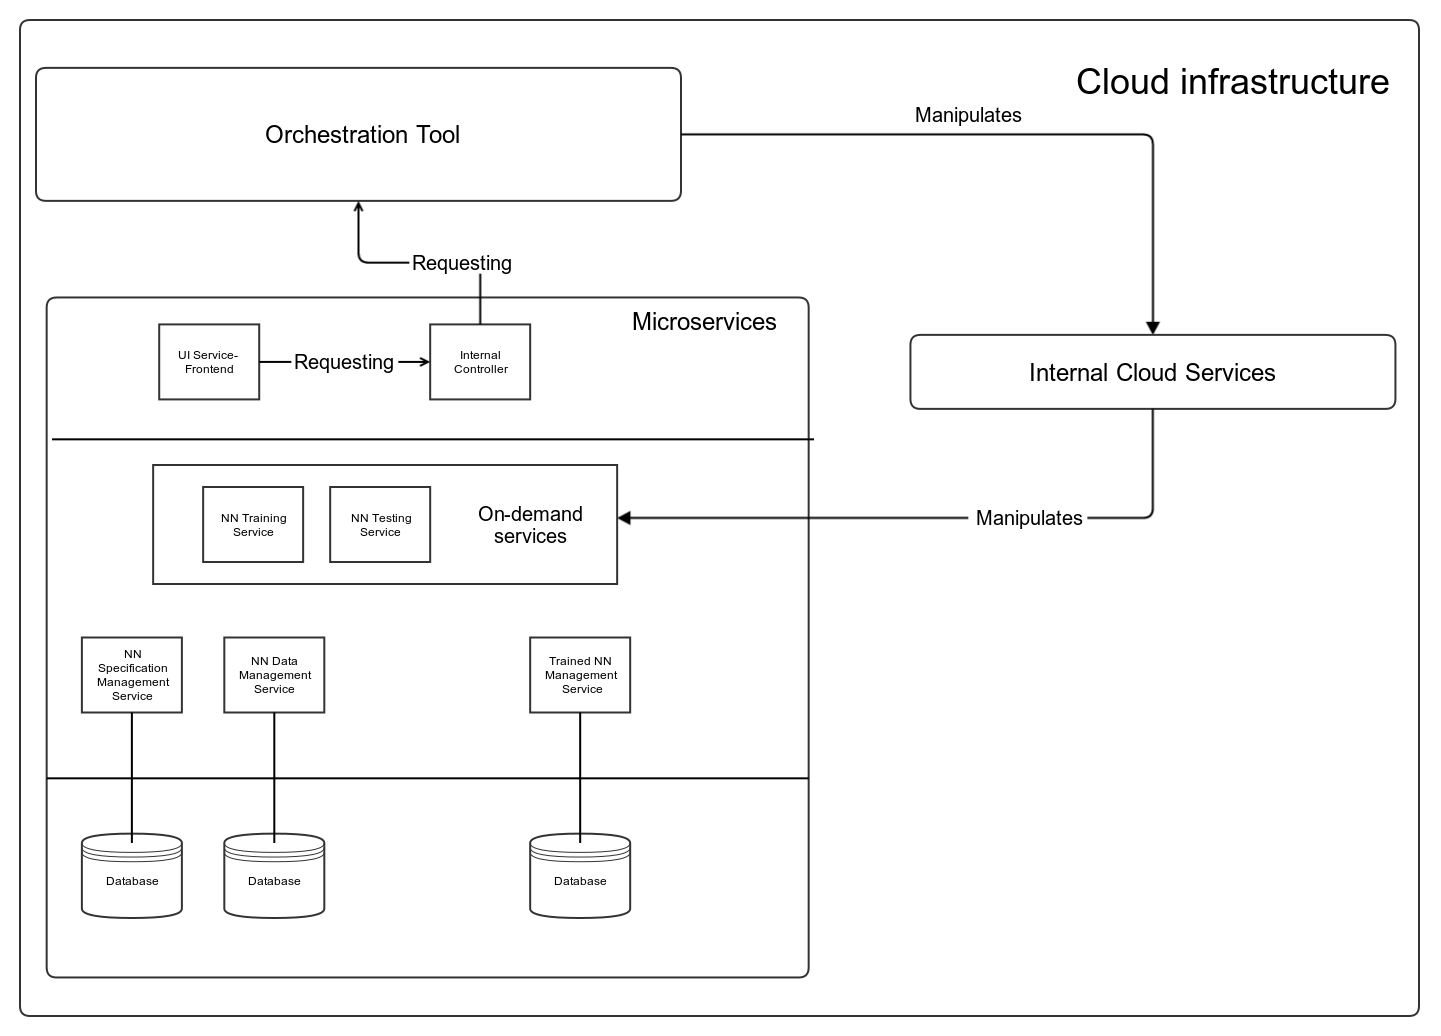
\includegraphics[width=\linewidth]{components/2/architecture.png}
  \caption{Novel N2Sky Architecture}
  \label{fig:newarch}
\end{center}
\end{figure}

\begin{itemize}
\item \emph{Orchestration Tool} is the Cloudify framework, which communicates with a cloud infrastructure namely create and manage new instances. Every instance is a Docker container.
\item \emph{Internal Controller} is a service, which works directly with the Cloudify tool. This service handles user request in order to create, delete or update Docker container.
\item \emph{UI Service-Frontend} is a modular application namely it is the Administration Module. The user over UI can request container management, which will be redirected to Internal Controller.
\item \emph{On-demand services} are not exposed publicly services, which can be controlled only by internal web services.  This approach helps to encapsulate the services pool, which increases security in the entire application. 
\item \emph{Neural Network Specification Management Service}  is a service, which is responsible for controlling existing neural network paradigms, namely train, retrain and persist trained models.
\item \emph{Neural Network Data Management Service}, this service located right on top of the database and provides API for adding external data sources.
\item \emph{Trained Neural Network Management Service} is a service, which responsible for evaluating trained models.
\end{itemize}


 
 
\subsubsection{Modular frontend application design}\label{Modular frontend application design}

Maintain large application like N2Sky with the monolithic approach is unwieldy. Since N2Sky supports microservices approach in the backend it was decided to apply the same solution on the frontend.  

Microservices in frontend are small independent web applications, which are consolidated into one application. The main benefits of this approach are:

\begin{itemize}
\item \emph{Maintainability.} It is possible to divide application between different teams. Developers do not even need to have some knowledge about other parts of the application. 
\item \emph{Diversity of technologies.} Monolithic approach makes the whole application stick to one framework. Microservices allowing to use any technology without the need to rewriting the application.
\item \emph{Independent deployment.} Every application has some releases periods, every release accompanies with redeployment procedure. There is no need to redeploy the whole application, but just only required components.
\end{itemize}


\begin{figure}[htbp]
\begin{center}
  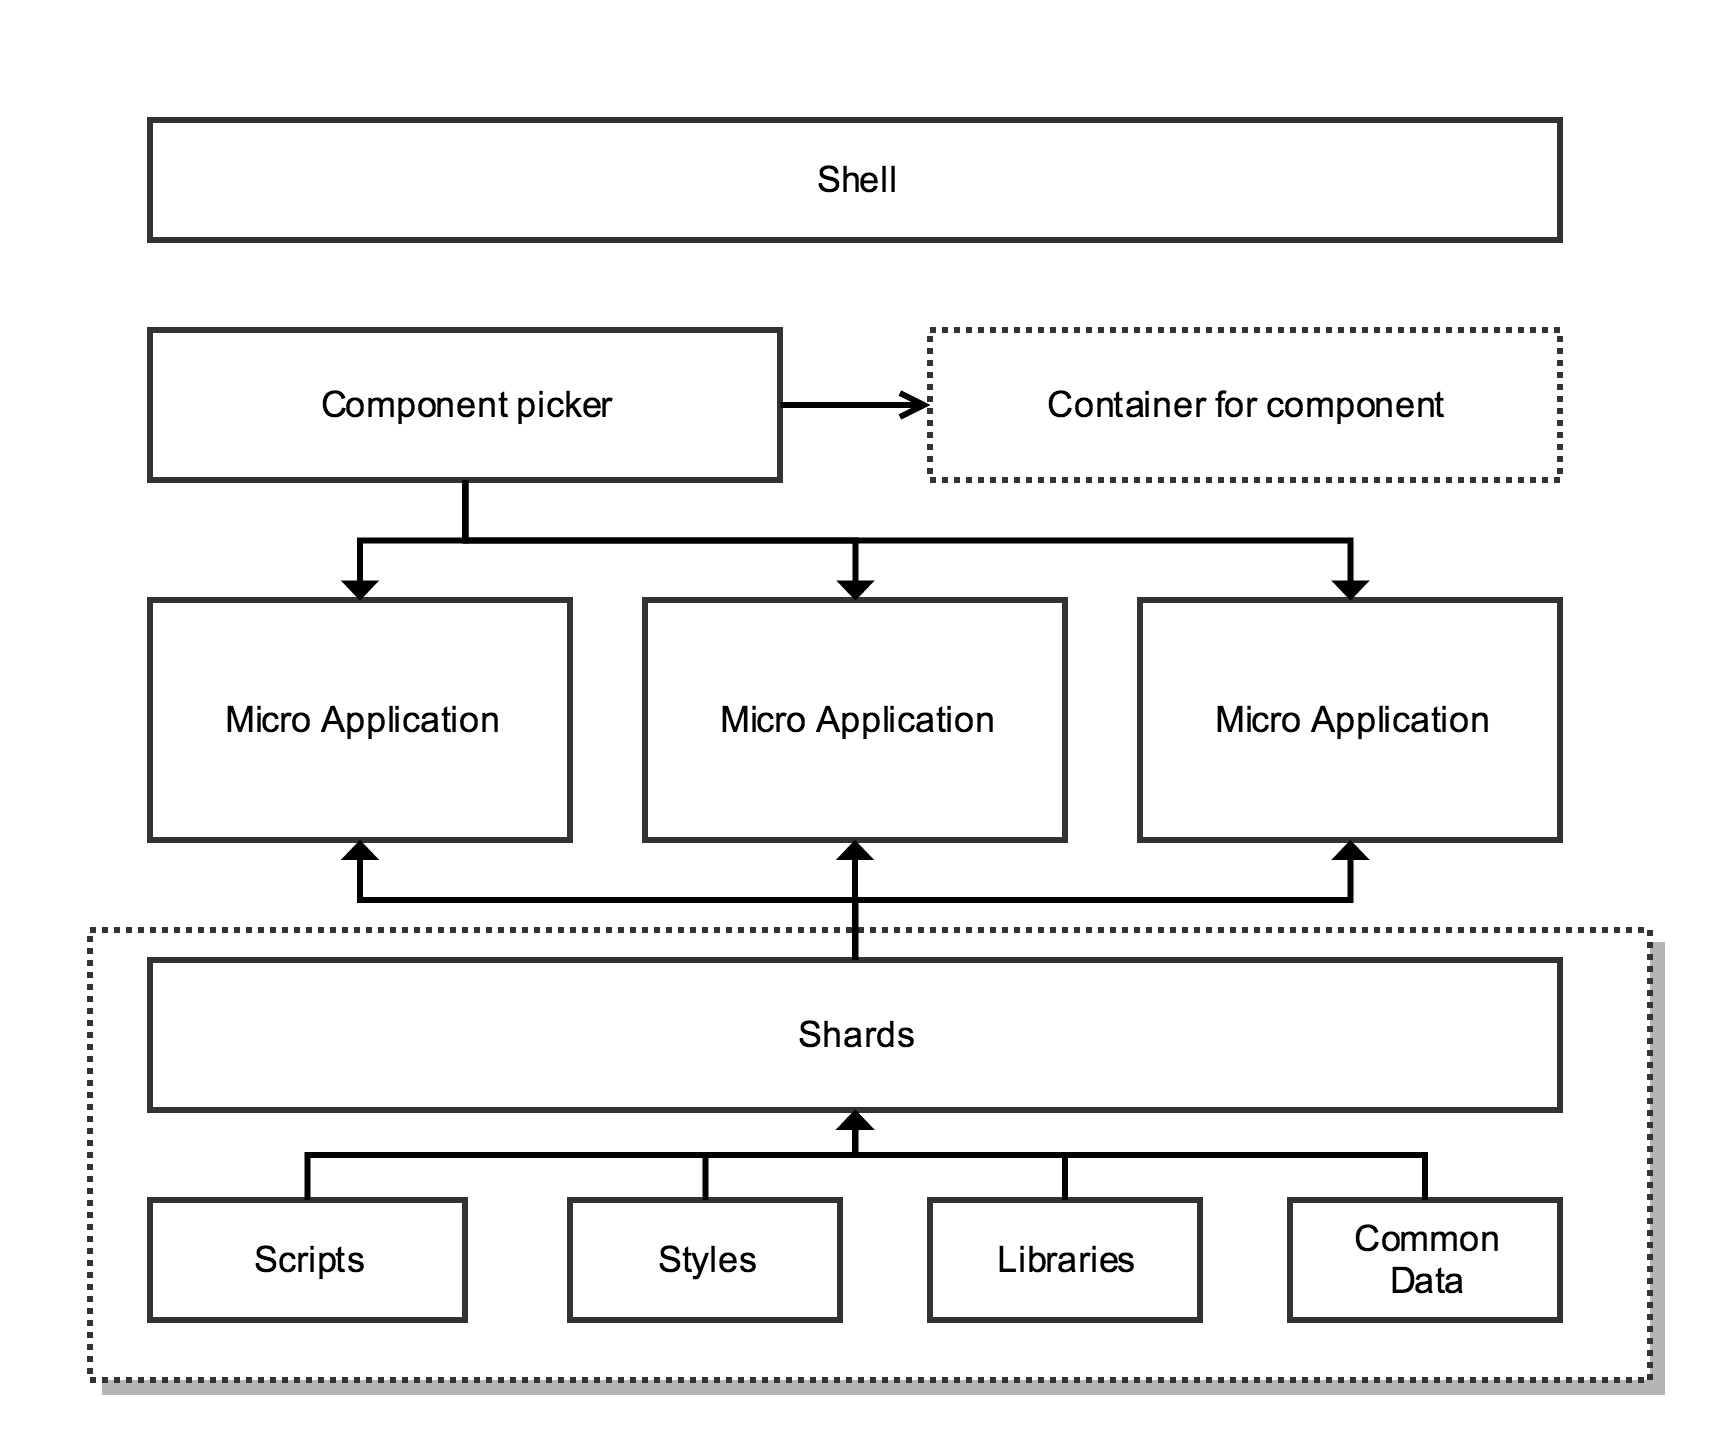
\includegraphics[width=\linewidth]{components/2/frontend_arch.png}
  \caption{Microservices approach in frontend application}
  \label{fig:frontend_arch}
\end{center}
\end{figure}


Microservices approach in frontend application is shown in ``Fig.~\ref{fig:frontend_arch}''. This breaks the entire application into small micro applications.

\begin{itemize}
\item \emph{Shell.}  is a top-level component, which wraps Components picker and Container for the component. It contains application configuration.
\item \emph{Component picker.} Is a router, which manages the micro applications. 
\item \emph{Container for Component.} Container, where the component will be injected.
\item \emph{Micro Application.} Independent application, which can be written in any programming language but has to use one of the shards.
\item \emph{Shards.} Is a code base, which is shared between Micro Applications. Shards can have multiple levels. 
\end{itemize}
 

The central concept of the application is to support the Software as a Service (SaaS) and Platform as a Service (PaaS) distributions \cite{Walraven2014}.  N2Sky consists of two modules: administration module, main application module as it shown in ``Fig.~\ref{fig:modular_design}''.

\begin{figure}[htbp]
\begin{center}
  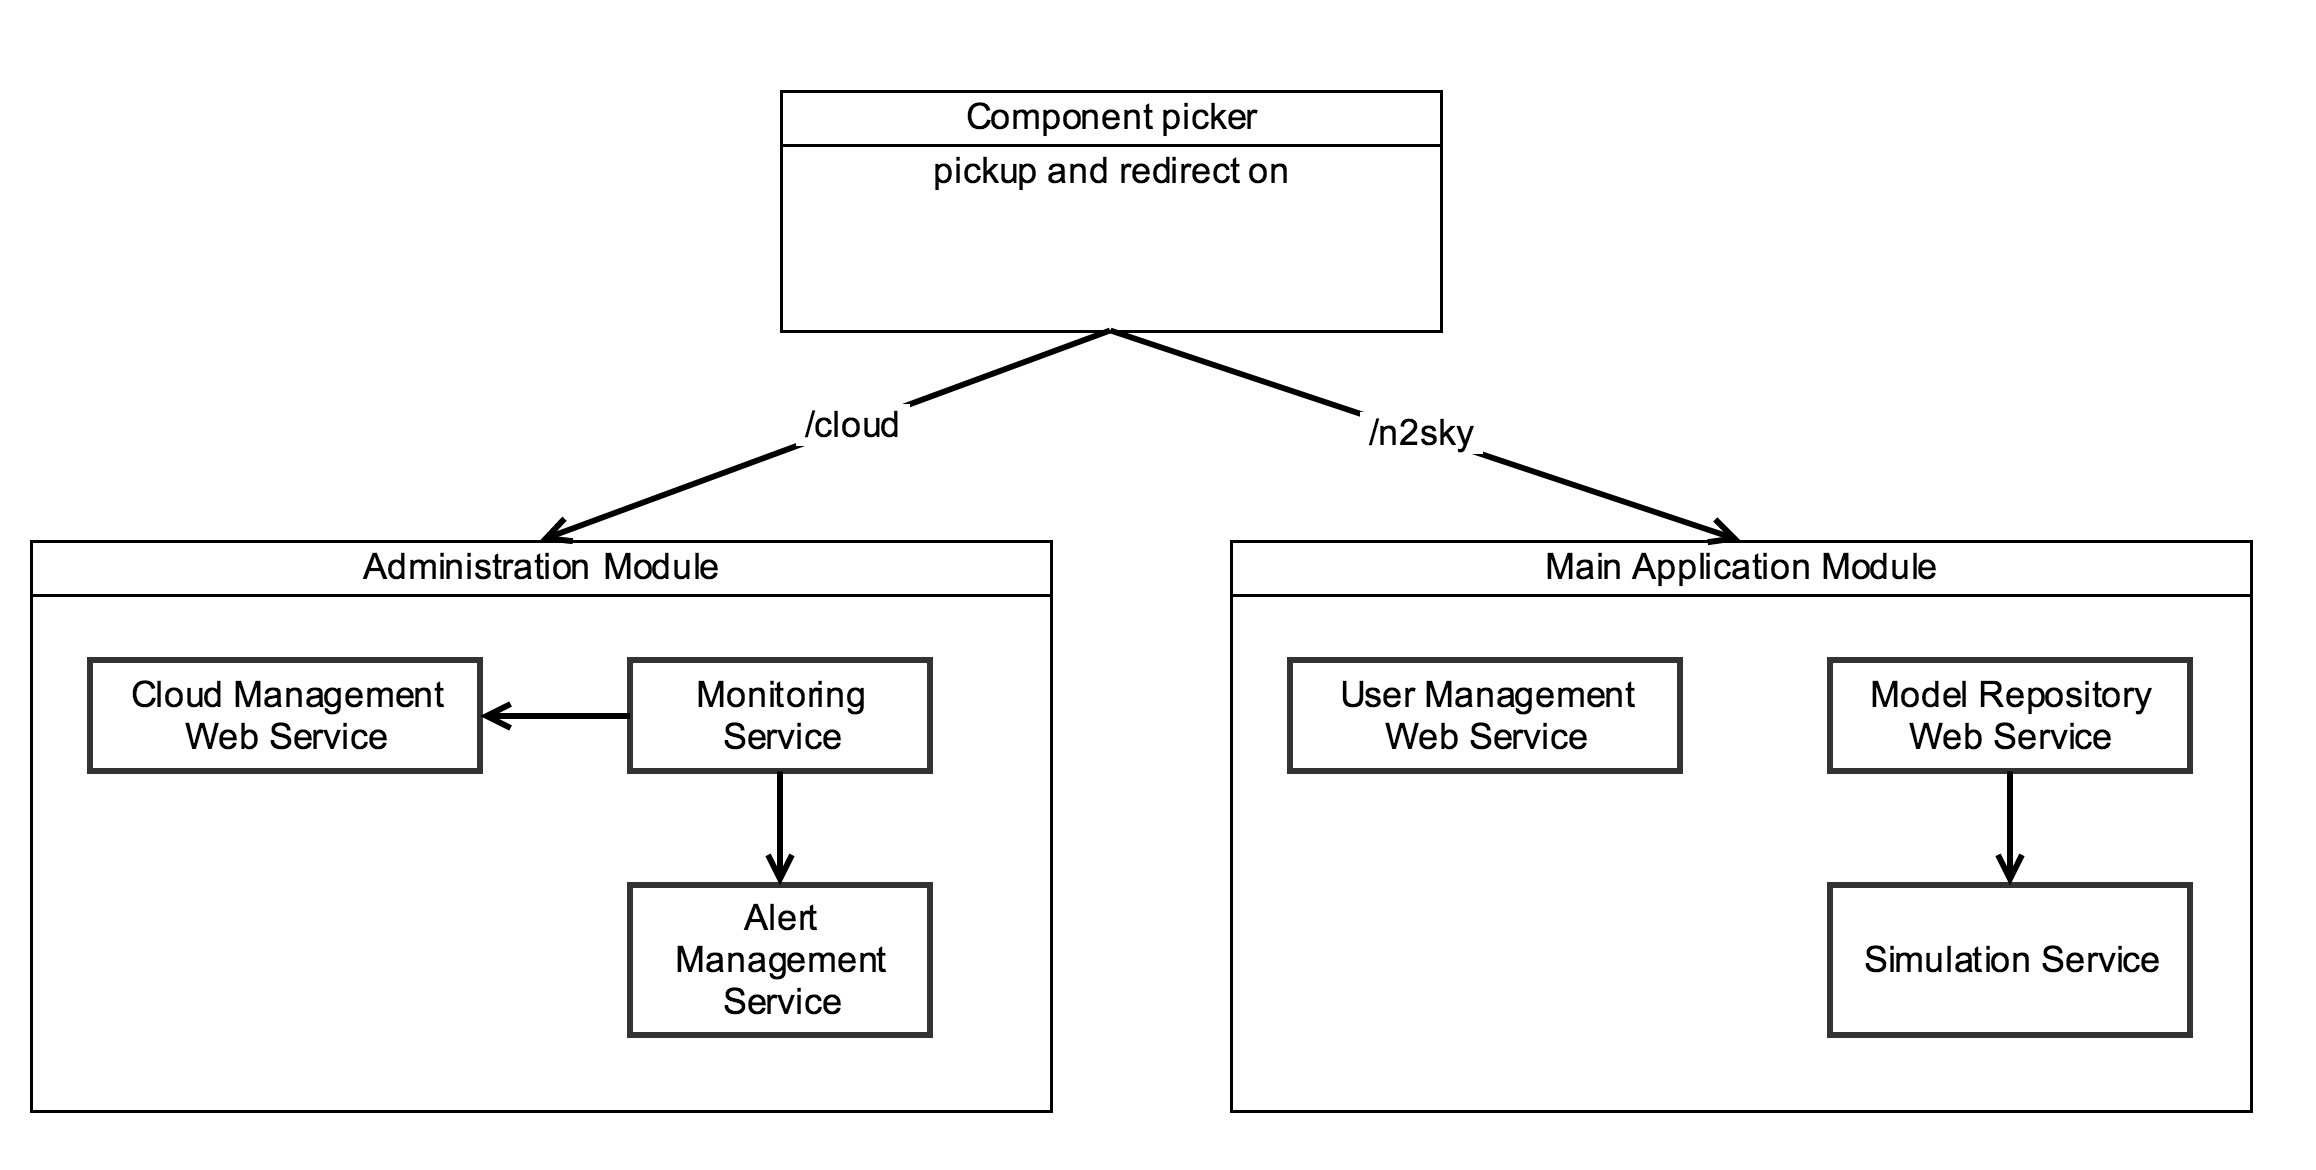
\includegraphics[width=\linewidth]{components/2/redirector.png}
  \caption{N2Sky frontend application and its services}
  \label{fig:modular_design}
\end{center}
\end{figure}

\begin{itemize}
\item \emph{N2Sky component picker.} When the user goes to N2Sky web portal, first he will be dealing with a component picker. The component picker is a small service, which redirects the user depending on URL path.
\begin{itemize}
\item \emph{/cloud} redirects to "Administration module"
\item \emph{/n2sky} redirects to "Main application module"
\end{itemize}


\item \emph{Administration module} The administration module allows the system administrator to control the environment. The module supports OpenStack and Cloudify monitoring. Managing is possible through the application dashboard. It also contains custom monitoring and an alerting management system, which can be installed on any server within the N2Sky user interface. The administration module implements PaaS. It is fully configurable and wrapped into the open source project in order to make the module accessible to the third-party applications. 
\item \emph{Main application module} The main application module is the central module of N2Sky. Within this module, users can use, train and test existing neural networks. It is possible to reuse the neural network paradigms and create own neural network. N2Sky allows deploying own network and store data in the cloud. Module services are supporting the SaaS distribution. Experts can use an application directly through the N2Sky API or they can integrate N2Sky services into their own application. 
\end{itemize}


\subsubsection{The sample workflow}


The central figure is the N2Sky Web/Mobile portal. Is is frontend application of the N2Sky, which consist of modular subsystems. Since the frontend application has responsive design it supports desktop devices as well as mobile devices. 
To support Software as a Service distribution every web service can work independently. It means that the stakeholders can use N2Sky via web portal as well as use N2Sky API.
N2Sky API allows  stakeholders:

\begin{itemize}
\item Authorise in the System
\item Create new neural from existing paradigm
\item Deploy own neural network on N2Sky environment 
\item Perform training against own as well published neural network
\item Perform testing against trained models
\end{itemize}

Almost everything is available for arbitrary stakeholders, except cloud services. In order to cloud service as a service, the user has to install it on his own cloud environment. This approach supports Platform as a Service distribution. Cloud services only for system administrator and for granted users are available. 


\begin{figure}[htbp]
\begin{center}
  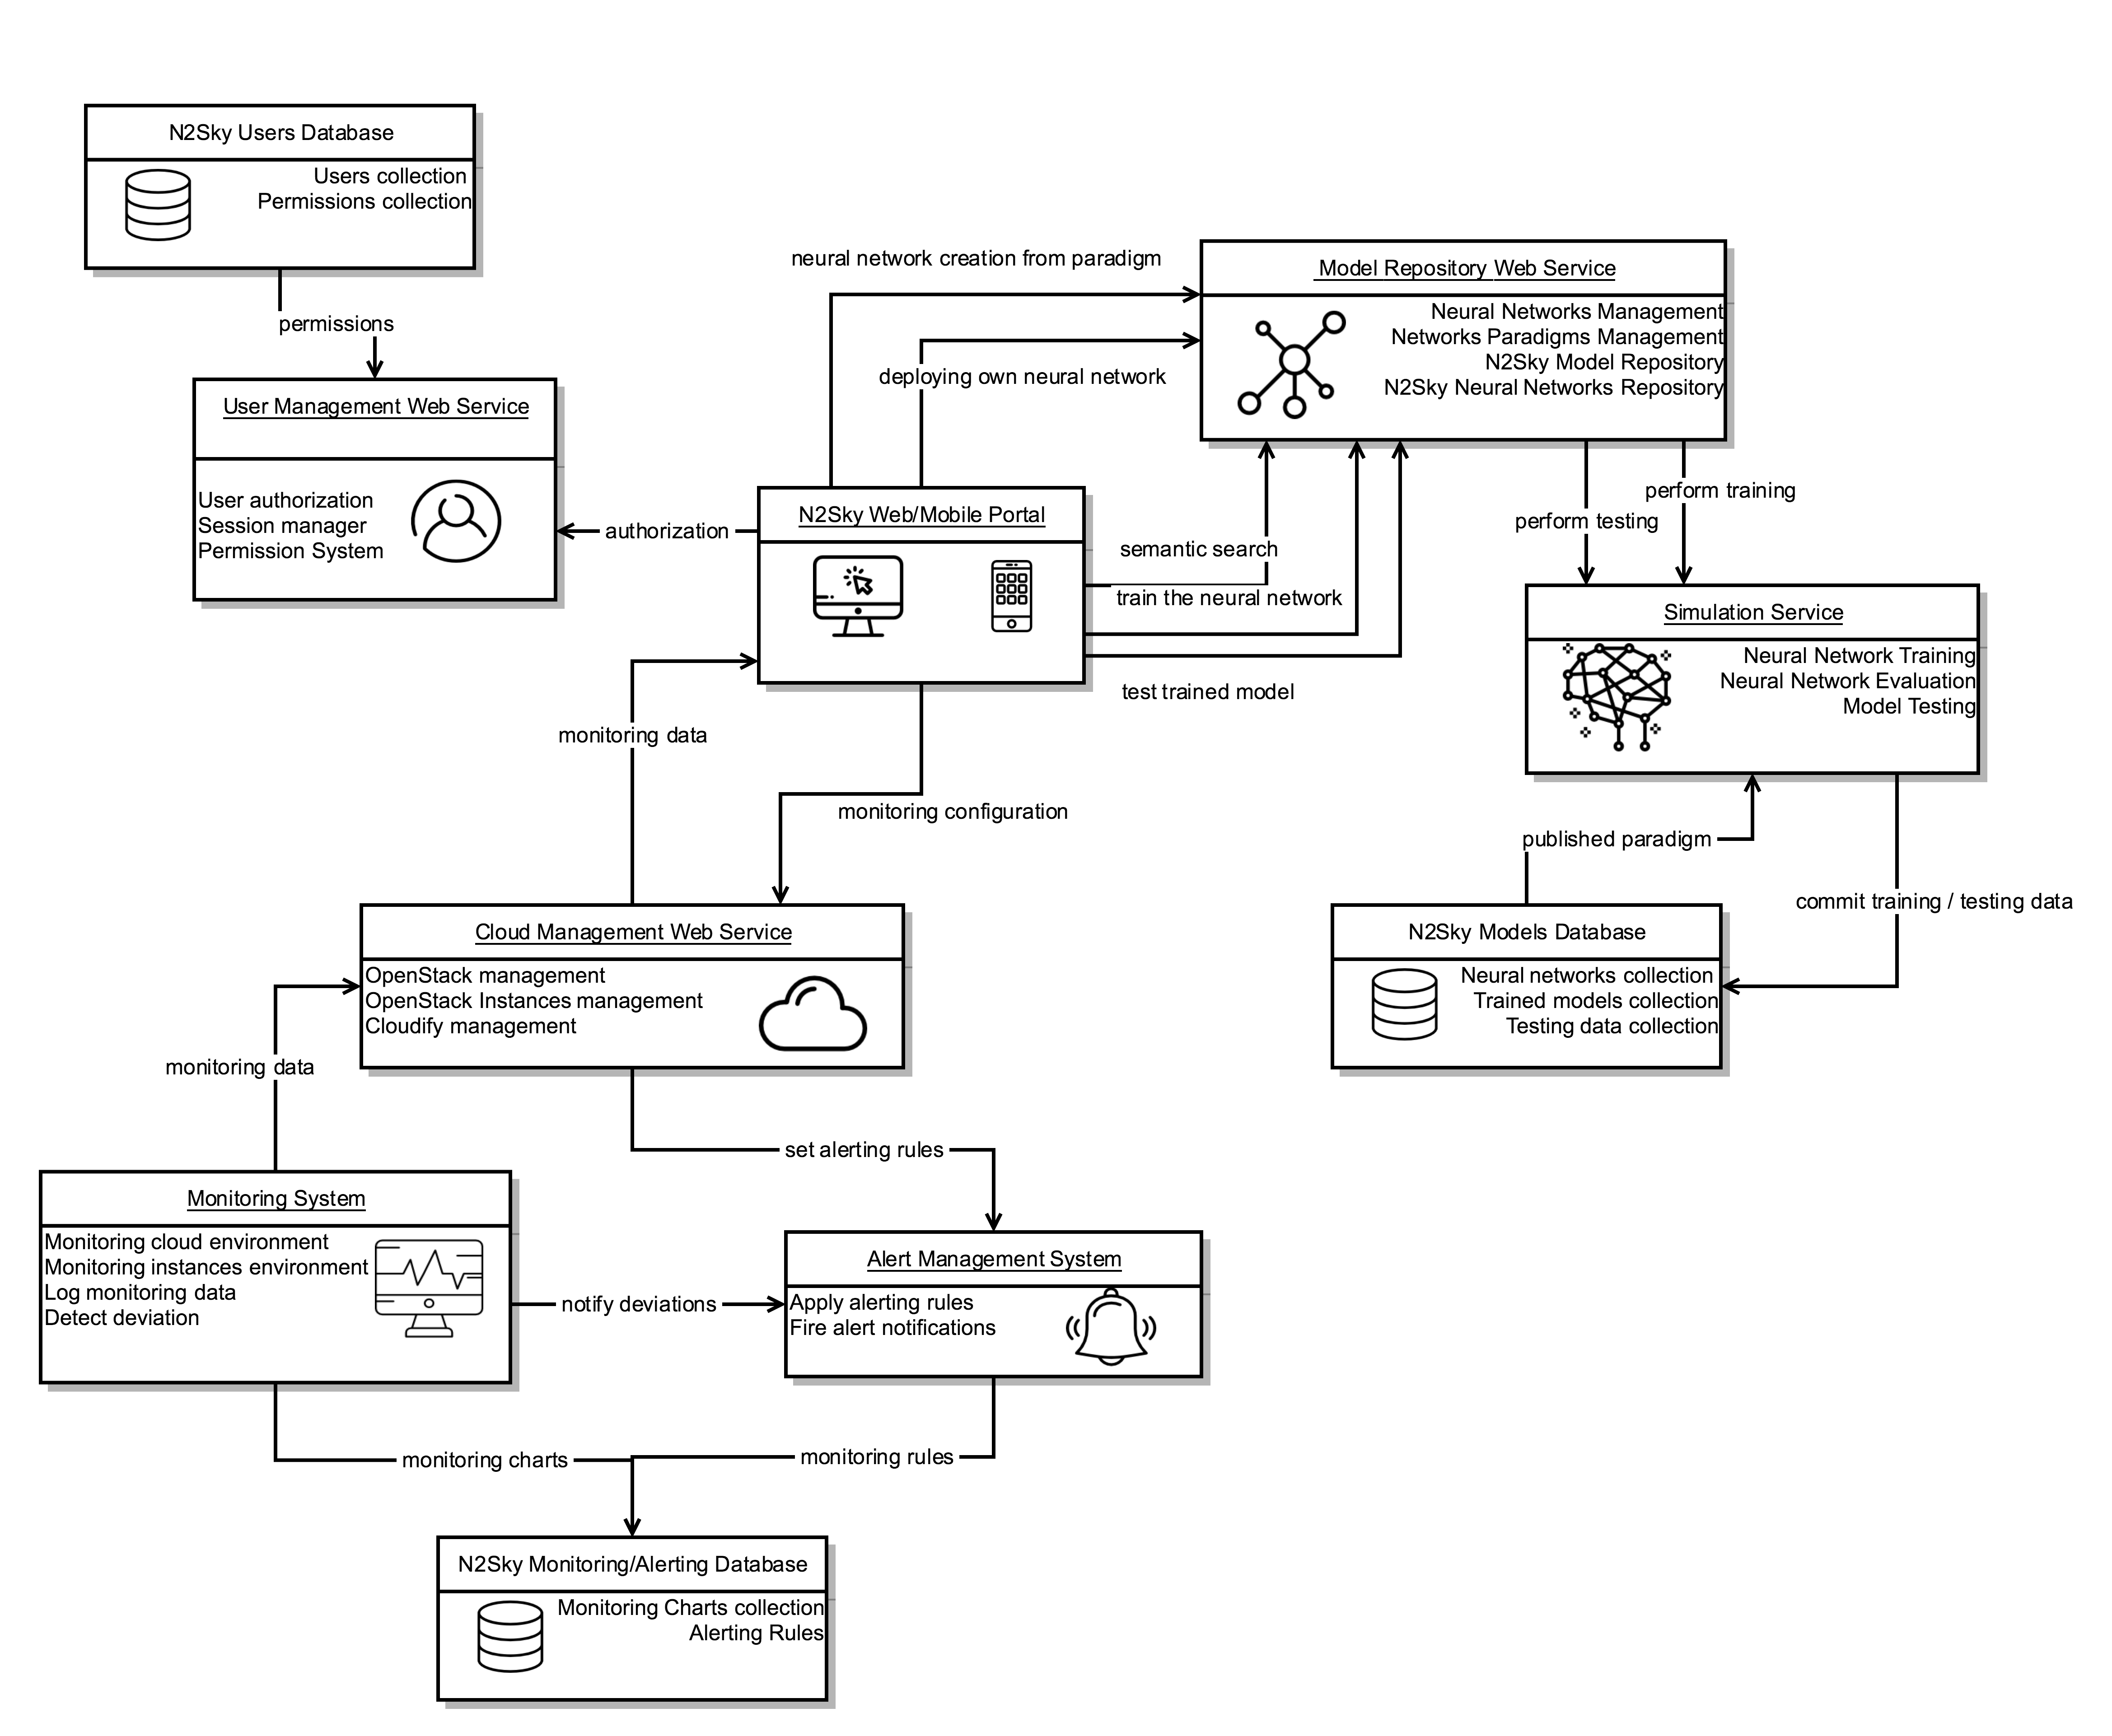
\includegraphics[width=\linewidth]{components/2/new_arch.png}
  \caption{The sample workflow}
  \label{fig:newarch}
\end{center}
\end{figure}


The sample workflow overview, which shown in ``Fig.~\ref{fig:newarch}'' represents microservices architecture in action:


\begin{enumerate}
\item \emph{Contributor User}
\begin{enumerate}
\item The Contributor user authorize in the N2Sky portal using his browser on desktop PC or mobile device. He will be redirected to his own dashboard according to permissions, which will be received from User Management Web Service. 
\item The user described his own neural network paradigm using the ViNNSL template and deploying it in the N2Sky cloud. 
\item The Contributor user perform training of his neural network using the N2Sky platform. Since the user is an expert he can perform this operation using Simulation Service via Model Repository Web Service API.
\item The user publishes his paradigm via N2Sky UI or available API. 
\item The Contributor user awaiting until other N2Sky users will use his neural network paradigm in order to monitor the behavior of the neural network. 
\item The user modify, redeploy and retrain his neural network after first results. 
\end{enumerate}
\item \emph{Neural Network Engineer User}
\begin{enumerate}
\item The neural network engineer user authorize in the N2Sky portal using his browser on desktop PC or mobile device. He will be redirected to his own dashboard according to permissions, which will be received from User Management Web Service. 
\item From the dashboard, the user creates a neural network from existing paradigm using Model Repository Web Service.
\item The user perform training against his newly created neural network using the N2Sky platform. 
\item If the user satisfied with a trained model he can perform testing using the N2Sky platform. 
\item The neural network engineer user publish his neural network and trained model in order to make it available for other N2Sky users. 
\end{enumerate}
\item \emph{Arbitrary User}
\begin{enumerate}
\item The arbitrary user authorize in the N2Sky portal using his browser on desktop PC or mobile device. He will be redirected to his own dashboard according to permissions, which will be received from User Management Web Service. 
\item Since the user does not much knowledge in neural network field, he performs a semantic search in order to find some neural network as well as trained models according to his needs.
\item The user copy existing neural network and some trained models into his project. 
\item The user perform training from N2Sky platform against copied neural network with the default input parameters data.
\item The user evaluate trained neural network model with the default parameters. 
\end{enumerate}
\item \emph{System Administrator}
\begin{enumerate}
\item The system administrator authorize in the N2Sky portal using his browser on desktop PC or mobile device. He will be redirected to administration dashboard.
\item The user observes cloud environment.
\item The system administrator creates the new monitoring chart with a specific metrics and add it to the administration dashboard.
\item The user creates alert against newly created monitoring
\item The user is notified by Alert Management System, that some event occurs.
\end{enumerate}
\end{enumerate}




 

\subsubsection{Technology Stack}\label{Technology Stack}

N2Sky today is the cross-platform handy application with a responsive design. Create own framework from scratch would be time consuming. To build cross-platform framework just for N2Sky is an absurd. After some research of most popular and common used frontend frameworks following candidates were listed: 

\begin{description}
\item[Vaadin.] Java framework, which compiles Java code into JavaScript components. Vaadin supports cross-platform application, but not fully. It is possible to wrap an applicaiton into container and deploy it only as an android application.

\begin{description}
\item[Benefits.] Easy to develop in Java. Developer does not have to think about JavaScript functionality. There are dozen of predefined components like: buttons, input fields, frames etc. Customisation is also possible. 
\item[Obstructions.] Deployment process is a blockage process. There is no "hot redeployment" available. Even if developer win some time by build components in Java, he will lose much more time by continuous redeployment. 

Java application need some server which supports JVM, it means that server should have much more memory then some other frameworks, which are written on JavaScript language.  
\end{description}

\item[ReactJS.]  JavaScript framework, which supports JSX programming language. 
\begin{description} 
\item[Benefits.] The main idea is to write HTML code in JavaScript. ReactJS supports hot redeployment.  React-Native extension for this framework, which allows to wrap the whole application mobile as well as desktop application.
\item[Obstructions.]  Difficult to support a big project. JSX is not a type safe programming language. Exception handling also need to be done by developer.  
\end{description}
\item[AngularJS.] JavaScript framework, which supports TypeScript programming language.
\begin{description} 
\item[Benefits.] The main idea is to write JavaScript code in HTML.  AngularJS same as ReactJS supports hot redeployment.  It does not have native support for all mobile devices, but is possible to wrap it using IONIC framework. 
\item[Obstructions.]  AngularJS compiles TypeScript code into JavaScript core and sometimes compilation fails because TypeScript is a new language and it is not fully adopted for browsers. 
\end{description}
\end{description}
 
 Vaadin does not fit N2Sky needs, but AngularJS and ReactJS could fit perfectly. Both of this frameworks are written on JavaScript and have big corporations behind: AngularJS was developed by Google and ReactJS was developed by Facebook. Since N2Sky has to support fully cross-platform architecture it was decided to choose ReactJS. With this framework N2Sky has a potential to be multi-platform application in the future. 
 

Furthermore, backend has microservices architecture to support scalability. After choosing JavaScript framework for frontend it will make sense to user JavaScript in a backend too, so that server would be small and fast. Each one of the microservices is developed on NodeJS Framework server, which implies efficiency and lightweight. 

N2Sky is a cloud-based system. OpenStack cloud platform supports this approach. Since N2Sky user OpenStack API for administration dashboard, the original OpenStack dashboard was no more needed. Every backend and frontend service is deployed on OpenStack instance. Every instance is absolutely scalable, which allows to find a best enviroment for every service. 

Every OpenStack instance is a server with either Debian or Ubuntu operational system. Every instance as well as OpenStack itself has to be monitored 24/7, that is why there was Monitoring Management System developed. The basis of this system is Prometheus monitoring system, which gives full access to all information of any server were its was installed. Prometheus has an open API, which is used by N2Sky. Using Prometheus there were charts and graphs developed and integrated into N2Sky. Alert Management System, which is a part of N2Sky, is also using  Prometheus API in order to detect deviation and notify on event occurred.

As a database it was decided to choose NoSQL one. There were two NoSQL databases under consideration ElasticSearch and MongoDB. 
ElasticSearch supports indexes. It is possible to configure index so, that is impossible to insert something which is not mapped by the index.  MongoDB does not user index approach, but MongoDB client supports schema. It was decided to use MongoDB schema and mapped ViNNSL schema to it in order to make it more understandable for other developers. 

For continuous delivery and quick configuration it was decided to use Jenkins Continuous Integration system. In case if the while system will go down it is possible to restore every service with a Jenkins Profiles.


